\documentclass[preview]{standalone}

\usepackage{amsmath}
\usepackage{amssymb}
\usepackage{tikz}
\usepackage{fancybox}
\usepackage{makecell}
\usepackage{stellar}
\usepackage{definitions}

\begin{document}

\id{merkle-tree}
\genpage

\section{Definition}

\begin{snippetdefinition}{merkle-tree-definition}{Merkle Tree}
    A Markle tree or hash tree is a tree where each node contains the hash
    of its children, and every leaf contains the hash of a data block.
\end{snippetdefinition}

\begin{snippetexample}{merkle-tree-example}{Merkle Tree}
    \begin{center}
        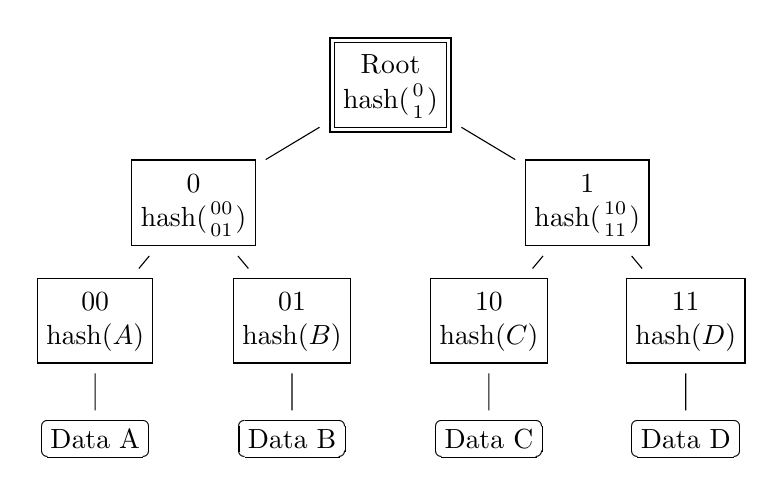
\begin{tikzpicture}[
            level 1/.style = {sibling distance = 5cm},
            level 2/.style = {sibling distance = 2.5cm}
        ]
        \node {\doublebox{\makecell{Root \\ \(\text{hash}({0\atop 1})\) }}}
            child {
                node {\fbox{\makecell{0 \\ \(\text{hash}({00\atop 01})\) }}}
                child {
                    node {\fbox{\makecell{00 \\ \(\text{hash}(A)\) }}}
                    child {
                        node {\ovalbox{Data A}}
                    }
                }
                child {
                    node {\fbox{\makecell{01 \\ \(\text{hash}(B)\) }}}
                    child {
                        node {\ovalbox{Data B}}
                    }
                }
            }
            child {
                node {\fbox{\makecell{1 \\ \(\text{hash}({10\atop 11})\) }}}
                child {
                    node {\fbox{\makecell{10 \\ \(\text{hash}(C)\) }}}
                    child {
                        node {\ovalbox{Data C}}
                    }
                }
                child {
                    node {\fbox{\makecell{11 \\ \(\text{hash}(D)\) }}}
                    child {
                        node {\ovalbox{Data D}}
                    }
                }
            };
        \end{tikzpicture}
    \end{center}
\end{snippetexample}

\end{document}
